\documentclass[%
%oneside,                 % oneside: electronic viewing, twoside: printing
%$final,                   % draft: marks overfull hboxes, figures with paths
10pt]{article}

\listfiles               %  print all files needed to compile this document

\usepackage{relsize,makeidx,color,setspace,amsmath,amsfonts,amssymb}
\usepackage[table]{xcolor}
\usepackage{bm,ltablex,microtype}
\usepackage{graphicx}

\usepackage[T1]{fontenc}
%\usepackage[latin1]{inputenc}
\usepackage{ucs}
\usepackage[utf8x]{inputenc}

\usepackage{lmodern}

% Hyperlinks in PDF:
\definecolor{linkcolor}{rgb}{0,0,0.4}
\usepackage{hyperref}
\hypersetup{
    breaklinks=true,
    colorlinks=true,
    linkcolor=linkcolor,
    urlcolor=linkcolor,
    citecolor=black,
    filecolor=black,
    %filecolor=blue,
    pdfmenubar=true,
    pdftoolbar=true,
    bookmarksdepth=3   % Uncomment (and tweak) for PDF bookmarks with more levels than the TOC
    }
%\hyperbaseurl{}   % hyperlinks are relative to this root

% Tricks for having figures close to where they are defined:
% 1. define less restrictive rules for where to put figures
\setcounter{topnumber}{2}
\setcounter{bottomnumber}{2}
\setcounter{totalnumber}{4}
\renewcommand{\topfraction}{0.95}
\renewcommand{\bottomfraction}{0.95}
\renewcommand{\textfraction}{0}
\renewcommand{\floatpagefraction}{0.75}
% floatpagefraction must always be less than topfraction!
% 2. ensure all figures are flushed before next section
\usepackage[section]{placeins}
% 3. enable begin{figure}[H] (often leads to ugly pagebreaks)
%\usepackage{float}\restylefloat{figure}

\usepackage[framemethod=TikZ]{mdframed}


\setcounter{secnumdepth}{3}
\setcounter{tocdepth}{3}
\begin{document}

\thispagestyle{empty}

\begin{center}
{\LARGE\bf
\begin{spacing}{1.25}
Machine Learning and Artificial Intelligence activities at FRIB
\end{spacing}
}
\end{center}

\tableofcontents
\newpage

\section{Explanation}


The purpose of this document is to collect information about the  competence  in the area of ML/AI at FRIB Laboratory. This is important, e.g., for the upcoming \href{https://www.jlab.org/conference/AI2020}{\it AI FOR NUCLEAR PHYSICS WORKSHOP} at JLab, March 4-6, 2020 and other related  activities.


\subsection{Description of individual entries}
Please format your entry (1 entry per page) according to the following template:

\vspace{5mm}
\noindent
\fbox{\begin{minipage}{0.98\linewidth}
{\bf Topic} (in subsubsection title)
\begin{description}
\item[Participants] List local faculty/staff, research associates (p), students (g,u), and external collaborators
\item[Description] Provide a short paragraph ($<$600 characters; think of a PRL abstract) describing the ML/AI work.
\item[FRIB relevance] ($<$600 characters) 
\item[Outcomes] List instrumentation outcomes, if any. Provide your published/submitted/anticipated papers with hyperlinks 
\end{description}
You are encouraged to provide a figure below the description.
\end{minipage}}

\section{Machine Learning and AI in Nuclear Physics}


Artificial intelligence (AI)-based techniques, particularly in machine
learning (ML) and optimization, are increasingly being used in many areas
of experimental and theoretical physics to facilitate discovery,
accelerate data analysis and modeling efforts, and bridge different
physical and temporal scales in numerical models.
The large amount of degrees of freedom pertain to both theory and experiment in nuclear physics. With increasingly complicated experiments that produce large amounts data, automated classification of events becomes increasingly important. 
Artificial intelligence and Machine Learning   techniques are proving to be powerful tools for advancing our
understanding of the physics from complicated nuclear systems. 



\subsection{Types of Machine Learning}



The approaches to machine learning are many, but are often split into two main categories. 
In \emph{supervised learning} we know the answer to a problem,
and let the computer deduce the logic behind it. On the other hand, \emph{unsupervised learning}
is a method for finding patterns and relationship in data sets without any prior knowledge of the system.
Some authors also operate with a third category, namely \emph{reinforcement learning}. This is a paradigm 
of learning inspired by behavioural psychology, where learning is achieved by trial-and-error, 
solely from rewards and punishment.

Another way to categorize machine learning tasks is to consider the desired output of a system.
Some of the most common tasks are:

\begin{itemize}
  \item Classification: Outputs are divided into two or more classes. The goal is to   produce a model that assigns inputs into one of these classes. An example is to identify  digits based on pictures of hand-written ones. Classification is typically supervised learning.

  \item Regression: Finding a functional relationship between an input data set and a reference data set.   The goal is to construct a function that maps input data to continuous output values.

  \item Clustering: Data are divided into groups with certain common traits, without knowing the different groups beforehand.  It is thus a form of unsupervised learning.
\end{itemize}
These categories are all part of the broad spectrum of AI and ML techniques being studied at FRIB. 


\subsection{Glossary of machine learning/statistical terms used}

We list here various acronyms used in the description of the different AI/ML projects.

\begin{description}
\item[AI] Artificial intelligence
\item[BMA] Bayesian Model Averaging
\item[CoD] Coefficient of determination
\item[GP] Gaussian processes
\item[MCMC] Markov chain Monte Carlo
\item[ML] Machine learning
\item[NN] Neural networks
\item[PCA] Principal component analysis and dimensionality Reduction Techniques
\item[UQ] Uncertainty quantification
\item[BM] Boltzmann Machines and Reduced Boltzmann Machines
\item[RNN] Recurrent Neural Networks
\item[CNN] Convolutional Neural Networks
\item[AE] Auto Encoders
\item[VAE] Variational Auto Encoders
\item[BML] Bayesian Machine Learning
\item[CL] Clustering
\item[LSTM] Long Short-Term Memory
\item[RL] Reinforcement Learning
\item[FS] Frequentist Statistics
\item[BS] Bayesian Statistics
\item[DRB] Decision Trees, Random Forests and Boosting
\item[SVM] Support Vector Machines
\item[LR] Logistic Regression
\item[REG] Linear Regression and beyond
\item[GM] Graphical Models
\end{description}

\section{AI/ML projects at FRIB}

\subsection{Accelerators}

\subsubsection{Add title}
\vspace{5mm}
\noindent
\fbox{\begin{minipage}{0.98\linewidth}
\begin{description}
%%%
\item[Participants:] Names%%%
\item[Description:]
%%%
\item[FRIB relevance:] 
%%%
\item[References:] {\it To be added}, in press/preparation/ or published 
\end{description}
%%%
\end{minipage}
}
\begin{figure}[htb!]
%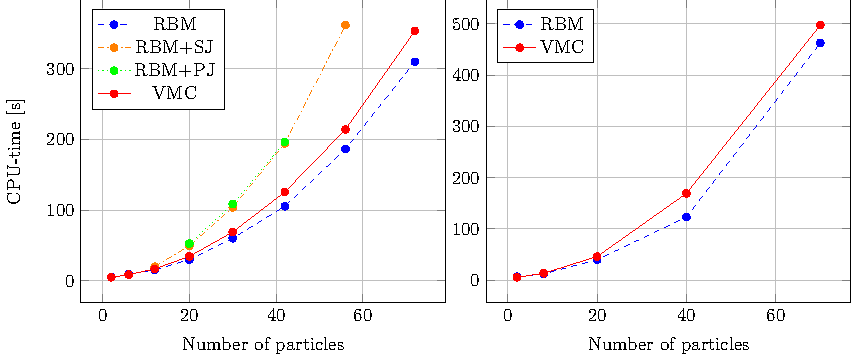
\includegraphics[width=\linewidth]{figures/quantumdots.pdf}
\caption{To be added}}
\end{figure}
\subsection{Detectors}
\subsubsection{Add title}
\vspace{5mm}
\noindent
\fbox{\begin{minipage}{0.98\linewidth}
\begin{description}
%%%
\item[Participants:] Names%%%
\item[Description:]
%%%
\item[FRIB relevance:] 
%%%
\item[References:] {\it To be added}, in press/preparation/ or published 
\end{description}
%%%
\end{minipage}
}
\begin{figure}[htb!]
%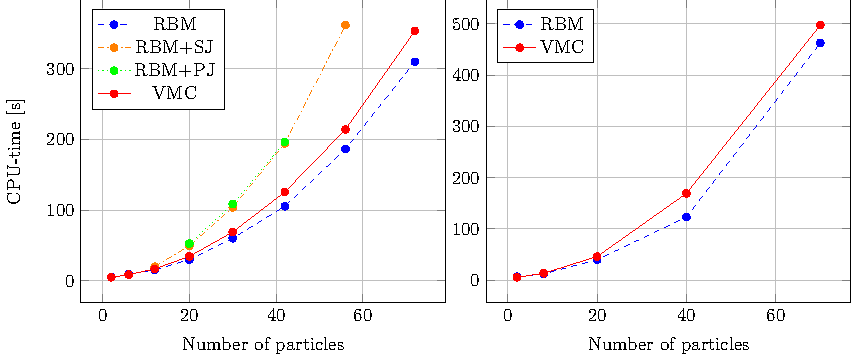
\includegraphics[width=\linewidth]{figures/quantumdots.pdf}
\caption{To be added}}
\end{figure}
\subsection{Data Analysis and Statistical Analysis}

\subsubsection{Add title}
\vspace{5mm}
\noindent
\fbox{\begin{minipage}{0.98\linewidth}
\begin{description}
%%%
\item[Participants:] 
%%%
\item[Description:]
%%%
\item[FRIB relevance:] 
%%%
\item[References:] {\it },
\end{description}
%%%
\end{minipage}
}
\begin{figure}[htb!]
%\includegraphics[width=\linewidth]{figures/rnnmbt.pdf}
\caption{To be added}
\end{figure}

\subsection{Basic Research}

\subsubsection{Quantified limits of the nuclear landscape}
\vspace{5mm}
\noindent
\fbox{\begin{minipage}{0.98\linewidth}
\begin{description}
%%%
\item[Participants:] L. Neufcourt (p), Y. Cao (g), S.A. Giuliani (p), W. Nazarewicz, O.B. Tarasov, and E. Olsen (ULB)
%%%
\item[Description:] We use microscopic nuclear global mass models and Bayesian methodology to provide quantified predictions of proton and neutron separation energies  as well as Bayesian probabilities of existence
 throughout the nuclear landscape all the way to the particle drip lines. To account for uncertainties, Bayesian GP are trained on the separation-energy residuals for each individual model, and the resulting  predictions are  combined via BMA. This framework allows to account for systematic and statistical uncertainties and propagate them to extrapolative predictions. 
%%%
\item[FRIB relevance:] Considering the anticipated  FRIB production rates and uncertainties of theoretical predictions, we identified  regions, reached by FRIB, that are crucial for constraining theoretical mass models.
%%%
\item[References:] {\it Beyond the proton drip line: Bayesian analysis of proton-emitting nuclei}, \href{https://journals.aps.org/prc/abstract/10.1103/PhysRevC.101.014319}{Phys. Rev. C 101, 014319 (2020)}; {\it Quantified limits of the nuclear landscape}, \href{https://arxiv.org/abs/2001.05924}{arXiv:2001.05924, submitted}.
\end{description}
%%%
\end{minipage}
}
\begin{figure}[htb!]
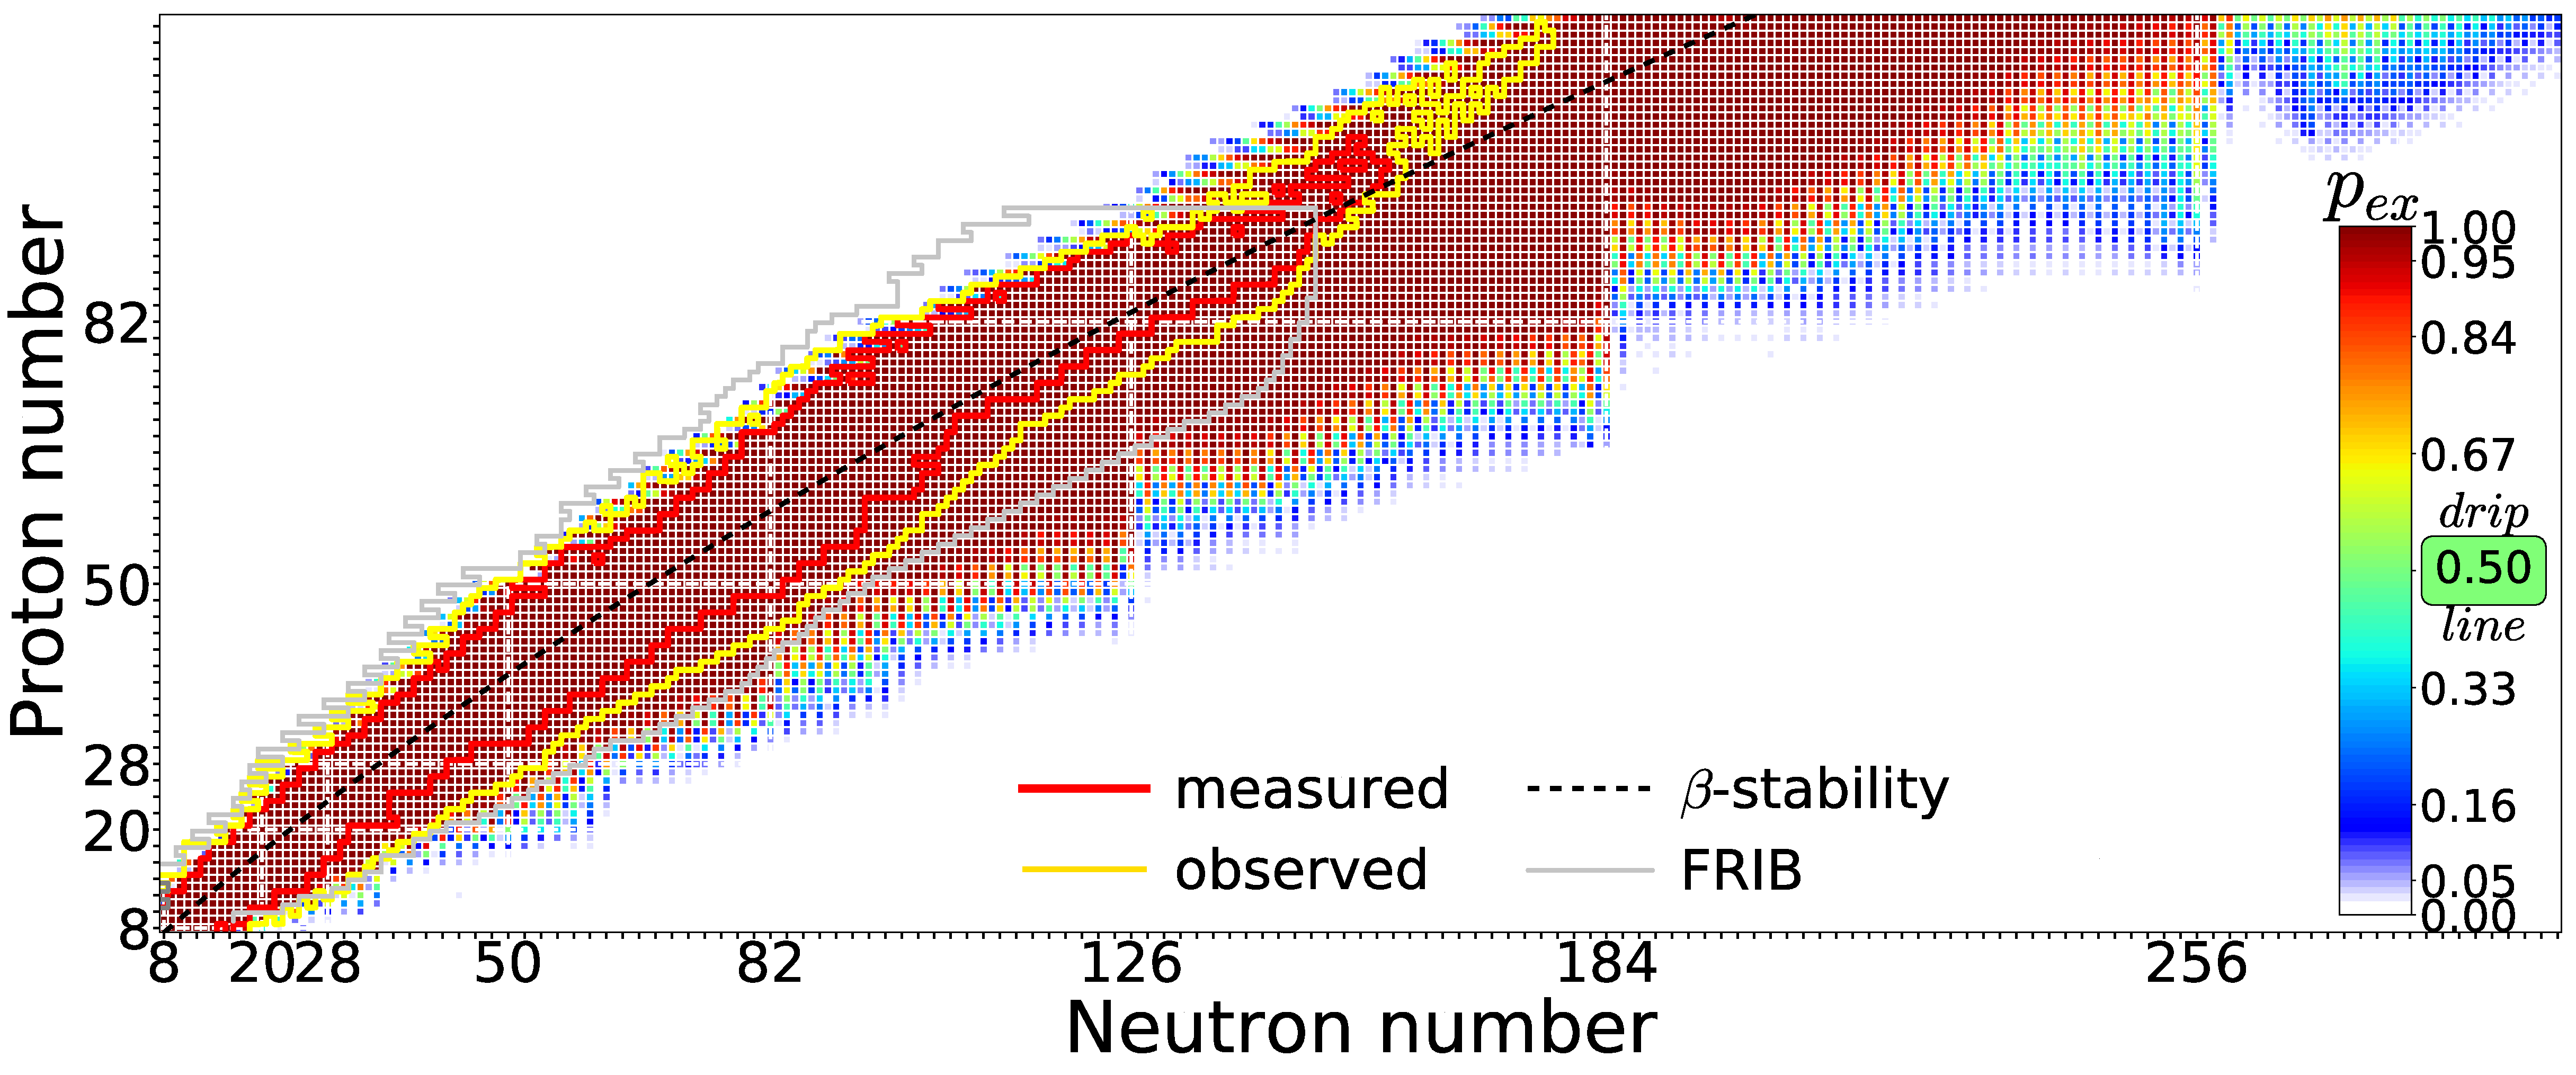
\includegraphics[width=\linewidth]{figures/Landscape.pdf}
\caption{
The quantified  landscape of nuclear existence obtained in our BMA calculations. For every nucleus with $Z,N \ge 8$ and $Z\le 119$
the probability that  the nucleus is bound with respect to proton and neutron decay, is marked.
The domains of nuclei which have been experimentally observed and whose separation energies have been  measured (and  used for training) are indicated together with 
the experimental reach of  FRIB.
}
\end{figure}
%%%%%%%%%%%%%%%%%%%%%%  Entry Ends %%%%%%%%%%%%%%%%%%%%%%%%%



\subsubsection{Deep Learning and the Nuclear Many-Body Problem}
\vspace{5mm}
\noindent
\fbox{\begin{minipage}{0.98\linewidth}
\begin{description}
%%%
\item[Participants:] J. Butler (g), Jane Kim (g), O Udiani (g), S. Bogner, H. Hergert and M Hjorth-Jensen
%%%
\item[Description:] Machine Learning based methods offer several possibilities to
circumvent the curse of  increasing dimensionality, as well as
allowing us to model quantum mechanical systems with less a priori
knowledge. For complex many-body systems like those which arise in
nuclear physics (in particular with the increase in the number of
degrees of freedom for nuclei close to their limits of stability), this is a very interesting avenue to explore.   We have recently explored  the solution of the Similarity
Renormalization Group set of equations using deep learning algorithms, with a great deal of success using RNNs and LSTM based approaches, as well as Kernel based methods. Preliminary studies of infinite nuclear matters holds great promise for handling systems of large numbers of particles.
%%%
\item[FRIB relevance:]  The ability to study theoretically nuclei at the limits of stability is a great challenge due to the increased number of degrees of freedom. These systems are highly relevant for the scientific program of FRIB. 
%%%
\item[References:] {\it Recurrent Neural Networks and the Nuclear Many-body Problem}, in preparation
\end{description}
%%%
\end{minipage}
}
\begin{figure}[htb!]
%\includegraphics[width=\linewidth]{figures/rnnmbt.pdf}
\caption{To be added}
\end{figure}






\subsection{Applications}


\section{Education and Work force development}

AI, ML, statistical data analysis and related areas are expected to
play an ever-increasing role in many areas, from fundamental and
applied research at universities and national laboratories to
applications and developments in both the private and the public
sectors.
Developing basic research activities in these frontier
computational technologies is thus of strategic importance for our
society’s capability to address future scientific problems. Transfer
of knowledge to other disciplines and sectors, as well as developing
lasting collaborations with partners outside the traditional
university sector, are themes we expect will benefit society at large
and that will play central roles. Nuclear Physics keeps attracting many brilliant young researchers and providing our work force with these competences and skills for solving complicated physics problems is a compelling task for our community.


\begin{itemize}
\item
We initiated the series of meetings on {\it Enhancing the interaction between nuclear experiment and theory through information and statistics} \href{https://iopscience.iop.org/journal/0954-3899/page/ISNET}{(ISNET)}.  The next ISNET-8 will be held at FRIB during  Dec. 14-17th, 2020.

\item In order to develop education and training efforts that target AI and ML related methods applied to Nuclear Physics, we  organized in 2019 a four day long  FRIB-TA workshop on ML methods in Nuclear physics at the NSCL/FRIB, with more than 100 participants.

\item In 2020 several of us (Bazin, Hjorth-Jensen and Liddick) will teach a three-week long Nuclear Talent course on Machine Learning and Data Analysis applied to nuclear physics. 

\item ISNET conferences
\end{itemize}








\end{document}
